\documentclass[xcolor=x11names,compress]{beamer}
\usepackage[english]{babel}

%% General document %%%%%%%%%%%%%%%%%%%%%%%%%%%%%%%%%%
\usepackage{graphicx}
\usepackage{tikz}
\usetikzlibrary{decorations.fractals}
%%%%%%%%%%%%%%%%%%%%%%%%%%%%%%%%%%%%%%%%%%%%%%%%%%%%%%


%% Beamer Layout %%%%%%%%%%%%%%%%%%%%%%%%%%%%%%%%%%
\useoutertheme[subsection=false,shadow]{miniframes}
\useinnertheme{default}
\usefonttheme{serif}
\usepackage{palatino}

\setbeamerfont{title like}{shape=\scshape}
\setbeamerfont{frametitle}{shape=\scshape}

\setbeamercolor*{lower separation line head}{bg=DeepSkyBlue4} 
\setbeamercolor*{normal text}{fg=black,bg=white} 
\setbeamercolor*{alerted text}{fg=red} 
\setbeamercolor*{example text}{fg=black} 
\setbeamercolor*{structure}{fg=black} 
 
\setbeamercolor*{palette tertiary}{fg=black,bg=black!10} 
\setbeamercolor*{palette quaternary}{fg=black,bg=black!10} 

\renewcommand{\(}{\begin{columns}}
\renewcommand{\)}{\end{columns}}
\newcommand{\<}[1]{\begin{column}{#1}}
\renewcommand{\>}{\end{column}}
%%%%%%%%%%%%%%%%%%%%%%%%%%%%%%%%%%%%%%%%%%%%%%%%%%



%\usepackage[english]{babel}
\usepackage[utf8]{inputenc}
%\usetheme{Goettingen}

\begin{document}
\title{Bifurcations in Dynamical systems with singularities}
\author{Debsankha Manik}
% - Give the names in the same order as the appear in the paper.
% - Use the \inst{?} command only if the authors have different
%   affiliation.


\begin{frame}

%opening

\titlepage

\end{frame}

\section{Definition}
\begin{frame}{Definition}
A simple piecewise smooth function:
\begin{displaymath}
   f(x) = \left\{
     \begin{array}{lr}
       g(x) & : x < \mu\\
       h(x) & : x > \mu
     \end{array}
   \right.
\end{displaymath}

Continuity demands $g(\mu)=h(\mu)$.  \\

\pause{}
Orger of singularity:\\
The power of the leading order term in the power series expansion of 
\[
g(x)-h(x)
\]
around $x=\mu$
\end{frame}


\section{Examples}
\begin{frame}
A system with singularity:\\
\begin{figure}
  \caption{}
  \begin{center}
    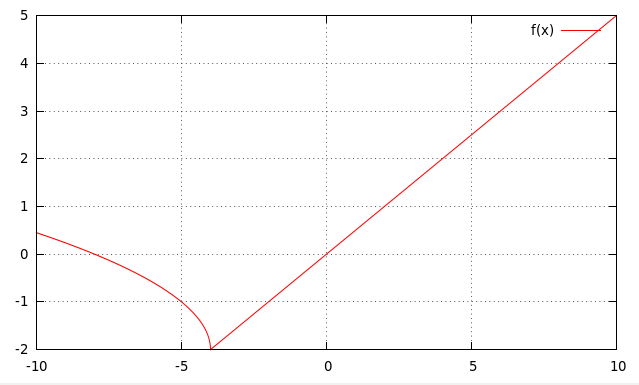
\includegraphics[width=0.5\columnwidth]{sq-sing}
  \end{center}
\end{figure}


\pause{}
\begin{displaymath}
   f(x) = \left\{
     \begin{array}{lr}
       \sqrt(\mu-x)-\mu\nu & : x<\mu\\
       \nu x & : x > \mu
     \end{array}
   \right.
\end{displaymath}

\[
g(\mu-x)-h(\mu-x)=\sqrt(x)+O(x)
\]

This is square root singularity.  
\end{frame}



\begin{frame}{Cobweb Diagrams}
\begin{figure}
  \caption{Cobweb Diagram}
  \begin{center}
    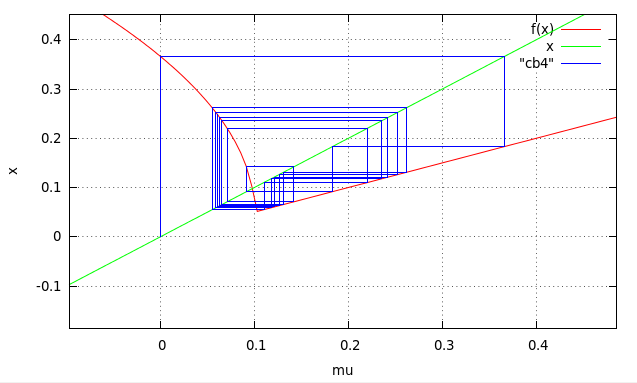
\includegraphics[width=0.9\columnwidth]{cb}
  \end{center}
\end{figure}
Attractor must be bounded.  

\end{frame}


\begin{frame}
For $\mu<0$, the stable fixed point is at $x=0$.  \\
Border collision occurs at $\mu=0$.  \\
What happens when $\mu$ crosses $0$ to positive values?\\
\pause{}

\begin{enumerate}
\item $\frac{2}{3}<\nu<1$: Immediate onset of chaos.  
\item $\frac{1}{4}<\nu<\frac{2}{3}$: There is a period-adding cascade as $mu$ 
decreases, with infinite-period orbits at $\mu=0$.  Moreover, chaotic regions 
between each $period m$ and $period m+1$ orbits.  
\item $0<\nu<\frac{1}{4}$: Periodic orbits.  
\end{enumerate}
\end{frame}


\section{Bifurcations}
\begin{frame}{Case 1: $\nu=0.12$}
\begin{figure}
  \caption{}
  \begin{center}
    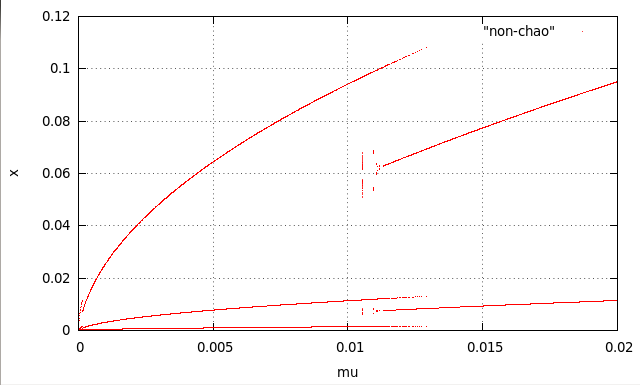
\includegraphics[width=0.9\columnwidth]{non-chao}
  \end{center}
\end{figure}
\end{frame}

\begin{frame}{Case 2: $\nu=0.5$}
\begin{figure}
  \caption{}
  \begin{center}
    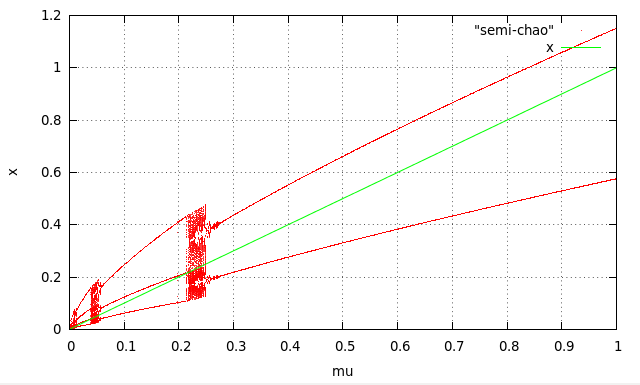
\includegraphics[width=0.9\columnwidth]{semi-chao}
  \end{center}
\end{figure}
\end{frame}

\begin{frame}{Case 3: $\nu=0.8$}
\begin{figure}
  \caption{}
  \begin{center}
    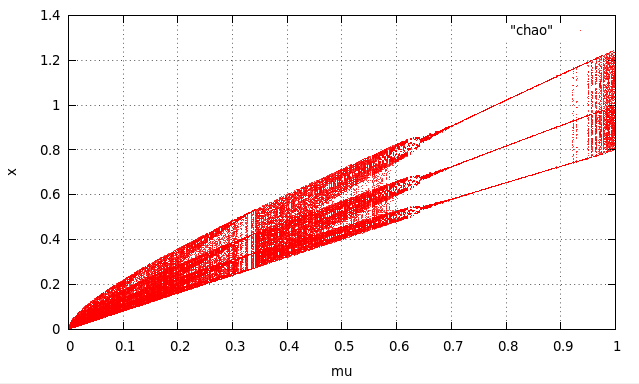
\includegraphics[width=0.9\columnwidth]{chao}
  \end{center}
\end{figure}
\end{frame}




\end{document}
